\section{Internal Combustion Engine Simulator}
%
ICESym es un simulador de motores de combustión de combustión interna que que
utiliza modelos 0D para la cámara de combustión y 1D para el flujo a través del
sistema de intercambio de gases.
%
Permite evaluar la \emph{performance} de un motor a un costo computacional bajo
además, la manera en que se implementó la entrada y salida de datos permite
utilizar el simulador como una \emph{caja negra} de modo que se pudo
implementar en un \emph{script} como una función a la que se le otorga un
conjunto de parámetros de entrada y devuelve los resultados de la simulación en
un formato que permite la lectura y evaluación de los mismos.
%

Se realizaron modificaciones menores al simulador, para facilitar la ejecución
en conjunto con el optimizador.
%
Algunas de estas modificaicones fueron:
\begin{enumerate}
    \item modificar los archivos de salida, eliminando valroes que no se
        utilizaron, de modo de reducir el tamaño de los archivos de salida,
        facilitar la lectura y el procesamiento de datos, 
    \item incluir una opción para elegir entre un modelo de $C_D$ de una o dos
        variables,
    \item modificar el área de referencia
    \item y  agregar una interpolación bilineal para podes trabajar con el mapa
        de $C_D$. 
\end{enumerate}

\section{Modificaciones a ICESym}
%%%%%%%%%%%%%%%%%%%%%%%%%%%%%%%%%%%%%%%%%%%%%%%%%%%%%%%%%%%%%%%%%%%%%%%%%%%%%%%
\subsection{Flujo a través de los puertos}
%
Para tener un mejor modelado del flujo de gas a través de los puertos de
admisión y escape, se introdujo una opción para poder ejecutar ICESym con un
modelo del coeficiente de descarga que dependa de dos variables, diferencia de
presión y \emph{alzada} o apertura del puerto $C_D = f(\Delta P; lv)$.
%
Esto significó agregar una opción que permita seleccionar entre un $C_D$ que
depende únicamente de una o dos variables.

Con esto se construye una mapa del coeficiente de descarga de la forma $C_D =
f(lv, dp)$, que se utiliza en \emph{def\_valve.f90} para calcular el área
efectiva de la válvula.

La interpolación bilineal se realiza sobre una malla rectangular, con esto se
realiza simplemente una interpolación lineal entre dos valores en planos con
datos conocidos.

% \begin{lstlisting}[language=fortran]
%    SUBROUTINE interpolant2d(x, y, z, xi, yi, zi)
%       [...]
%       nx = SIZE(x)
%       IF (xi .LE. x(1)) THEN ! <=
%          CALL interpolant(y, z(1, :), yi, zi)
%          RETURN
%       ELSE IF (xi .GE. x(nx)) THEN  ! >=
%          CALL interpolant(y, z(nx, :), yi, zi)
%          RETURN
%       END IF
%       i = iminloc(dabs(x - xi))
%       IF (x(i) .GT. xi) i = i - 1 ! >
%       CALL interpolant(y, z(i, :), yi, z_aux(1))   ! z1=f(x1,yi)
%       CALL interpolant(y, z(i + 1, :), yi, z_aux(2)) ! z2=f(x2,yi)
%       CALL interpolant(x(i:i + 1), z_aux, xi, zi)   ! zi=f(xi,yi)
%       [...]
%    END SUBROUTINE interpolant2d
% \end{lstlisting}

\begin{algorithm}
 \caption{Interpolación bi-lineal}\label{algo:bilineal}
    \SetAlgoLined
    \SetKwFunction{Size}{Size}
    \SetKwFunction{Interpolant}{Interpolant}

    \KwIn{\\
        $\vec{x}, \vec{y}$: valores de $x, y$ en los que se conoce el valor en $z$.\\
        $\vec{z}$: valores conocidos de $z$.\\
        $x_i, y_i$: puntos donde se quiere interpolar.\\
      }
    \KwResult{Devuelve el valor interpolado de $z_i$.}
    $n_x \Leftarrow Size(x)$\;
    \eIf{
      $x_i \geq x_{n_x}$
    }{
      $z_i \Leftarrow Interpolant(y, z[1,:], y_i)$\;
      \Return\;
    }{
      $z_i \Leftarrow Interpolant(y, z[n_x,:], y_i)$\;
      \Return\;
    }
    $i \Leftarrow iminloc(dabas(x-x_i))$\;

\end{algorithm}

Si bien hay otros métodos para estimar el valor de $C_D$ para dos valores $(\Delta
P; l_v)$, este método es sencillo y da resultados satisfactorios.
%
En la figura~\ref{fig:bilineal} se muestra un ejemplo del error obtenido con
este método para interpolar una función de prueba $\sin(\sqrt(x^2 + y^2))$.

\begin{figure}
    %
    \centering
    %
    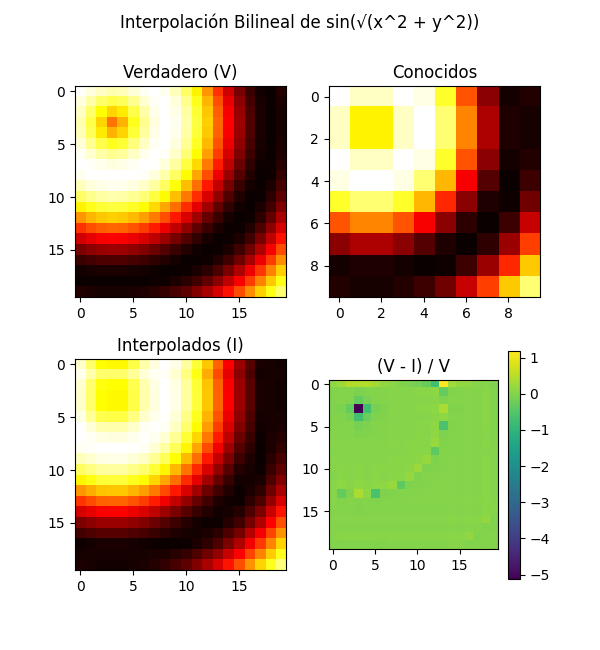
\includegraphics[width=0.7\textwidth]{bilineal.png}
    %
    \caption{Interpolación bilineal de $\sin(\sqrt(x^2 +
    y^2))$}\label{fig:bilineal}
    %
\end{figure}

La malla rectangular se realizará a partir de los valores de $C_D$ que se
obtengan de flujometrías con \emph{OpenFOAM}~\parencite{openfoam}.
%
Debido al costo computacional que requieren la flujometría, solo una cantidad
reducida de puntos se obtendrá con este método, las combinaciones de $(\Delta
P; l_v)$ ensayadas se indican con detalle en apartados posteriores.
%
Esto significa que se tiene como punto de partida una malla no rectangular, por
lo que se utiliza un método intermedio para obtener una matriz de puntos que
pueda ser leído por la interpolación bilineal.

Se probaron dos métodos para realizar la interpolación, el método del punto más
cercano y la interpolación por la suma de la inversa de la distancia o IDW por
sus siglas en inglés (\emph{Inverse Distance Weighting}).
%
Estos métodos se combinan con suavizados con un promedio móvil de los $n$
valores más cercanos.

El método del punto más cercano consiste en asignar para cada par $(x, y)$ el
valor conocido más cercano, el algoritmo es como se indica a continuación:

\begin{algorithm}
 \caption{Interpolación por punto más cercano}\label{algo:mas_cercano}
    \SetAlgoLined

    \KwIn{\\
        $V_x, V_y$: valores de $x, y$ en los que se conoce el valor en $z$.\\
        $V_z$: valores conocidos de $z$.\\
        $I_x$: $n$ puntos de $x$ donde se quiere interpolar\\
        $I_Y$: $m$ puntos de $y$ donde se quiere interpolar\\
        }

    \KwResult{Devuelve una matriz $I_{[n,m]}$ con los valores interpolados,
      donde cada punto $I(x,y)$ se le asigna al valor de $V_Z$ más cercano
      conocido. Da como resultado superficies escalonadas.}

    \BlankLine
     $I=zeros_{[n,m]}$\;
     \For{$i \gets 0$\KwTo$n$}{
        \For{$j \gets 0$\KwTo$m$}{
          $d = \sqrt{{(V_x - I_{xi})}^2 + {(V_y - I_{yj})}^2}$\;
            $I[i,j] = v_z[\min(d)]$\;
        }
     }
\end{algorithm}

La interpolación IDW consiste en asignar a cada punto el resultado de un
promedio de los valores cercanos al punto en cuestión, ponderado por la
distancia al valor elevado a un exponente arbitrario $p$.
%
Cuanto mayor sea el valor de $p$, más sensible es el método a los valores
cercanos, la formulación de este método se ve en la ecuación~\ref{eq:idw}.

\begin{equation}
    %
    f_p = \frac{\sum_{i=1}^{n} \frac{z_i}{d_i^p}} {\sum_{i=1}^{n}
    \frac{1}{d_i^p}}
    %
    \label{eq:idw}
    %
\end{equation}

La función utilizada para calcular esto es esto es:

\begin{algorithm}
    \caption{Interpolación IDW}\label{algo:IDW}
    \SetAlgoLined

    \KwIn{\\
        $V_x, V_y$: valores de $x, y$ en los que se conoce el valor en $z$.\\
        $V_z$: valores conocidos de $z$.\\
        $I_x$: $n$ puntos de $x$ donde se quiere interpolar\\
        $I_Y$: $m$ puntos de $y$ donde se quiere interpolar\\
        $p$: potencia a la que se eleva cada peso\\
        }

    \KwResult{Interpolación ponderada por inverso de la distancia. Dependiendo
      del valor de p, se obtienen valores más o menos suavizados.}

    \BlankLine
    $I=zeros_{[n,m]}$\;
    \For{$i \gets 0$\KwTo$n$}{
        \For{$j$\gets 0 \KwTo$m$}{
          $d = {\left[{(V_x - I_{xi})}^2 +{(V_y - I_{yj})}^2\right]}^{\frac{p}{2}}$\;
          \eIf{$\exists i : d[i] = 0$}{
            $I[i, j] = V_z[i]$\;
          }{
            $I[i,j] = \frac{\sum{V_{zi}/d_i}}{\sum \frac{1}{d}}$\;
          }
        }
     }
\end{algorithm}

\begin{figure}
    \centering
    \begin{subfigure}{0.4\textwidth}
        \centering
        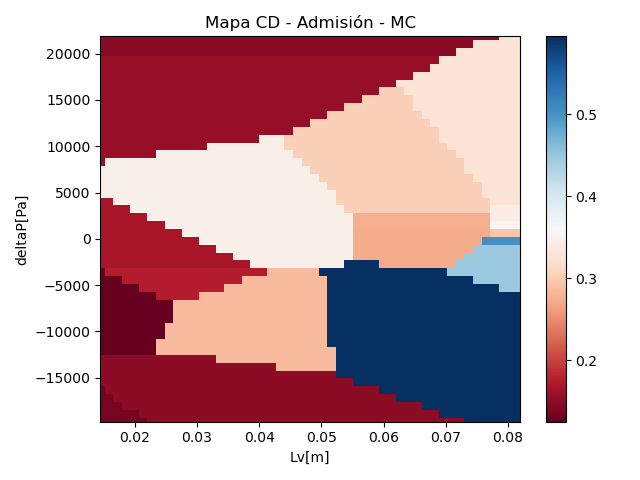
\includegraphics[width=\textwidth]{mapa_cd/mc_mapa_adm.png}
        \caption{Punto Más Cercano sin suavizar}
    \end{subfigure}
    \hfill
    \begin{subfigure}{0.4\textwidth}
        \centering
        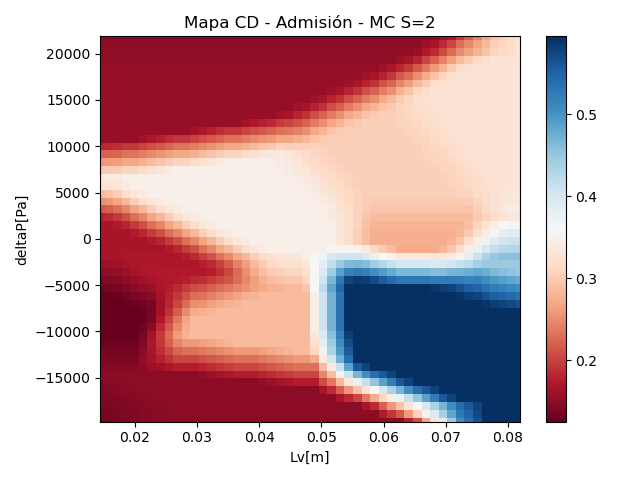
\includegraphics[width=\textwidth]{mapa_cd/mc_s2_mapa_adm.png}
        \caption{Más Cercano ($S=2$)}
    \end{subfigure}
    \hfill
    \begin{subfigure}{0.4\textwidth}
        \centering
        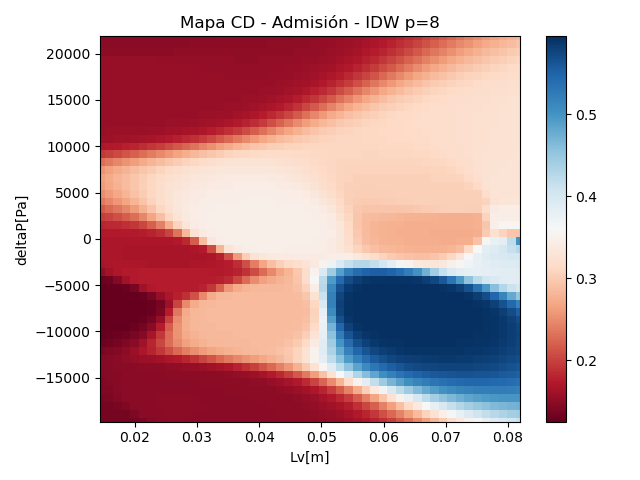
\includegraphics[width=\textwidth]{mapa_cd/idw8_mapa_adm.png}
        \caption{IDW ($p=8$)}
    \end{subfigure}
    \hfill
    \begin{subfigure}{0.4\textwidth}
        \centering
        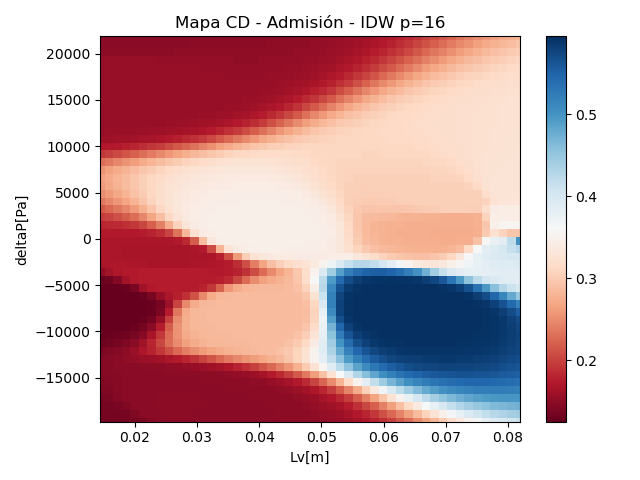
\includegraphics[width=\textwidth]{mapa_cd/idw16_mapa_adm.png}
        \caption{IDW ($p=16$)}
    \end{subfigure}
    \caption{Comparación de interpolaciones}\label{fig:mapas_interpolados}
\end{figure}

%%%%%%%%%%%%%%%%%%%%%%%%%%%%%%%%%%%%%%%%%%%%%%%%%%%%%%%%%%%%%%%%%%%%%%%%%%%%%%%

\subsection{Área de referencia}
%
El área de referencia utilizada por ICESym ese el área de
cortina~\ref{eq:area_cortina} y se expresa en el código del programa como el
área efectiva $F_{V}=A_{R}\cdot C_{D}$.
%
Para el MRCVC el área de referencia es el área frontal del puerto expuesta a la
cámara, calculada como la altura de la ranura $h_{p}$ multiplicada por la
longitud entre el borde del puerto y la paleta que delimita la cámara $l_{v}$,
$A_{R} = h_{p} \cdot l_{{v}}$.
%
En la figura~\ref{fig:area_referencia} se ilustran las áreas de referencia para
una posición del rotor en la que hay solape de cámaras con $\theta = 55^\circ$.
%
Este valor se afecta por el coeficiente de descarga $C_{D,int}$, puede ser un
valor fijo o el resultado de interpolar de un mapa de $C_D$ para un valor de
cuerda y $\Delta_P$ dado, esto en $m^2$ queda como:

\begin{equation}\label{eq:fv}
    %
    F_v = C_{D,int}*0.0294*l_v
    %
\end{equation}

\begin{figure}
    \centering
    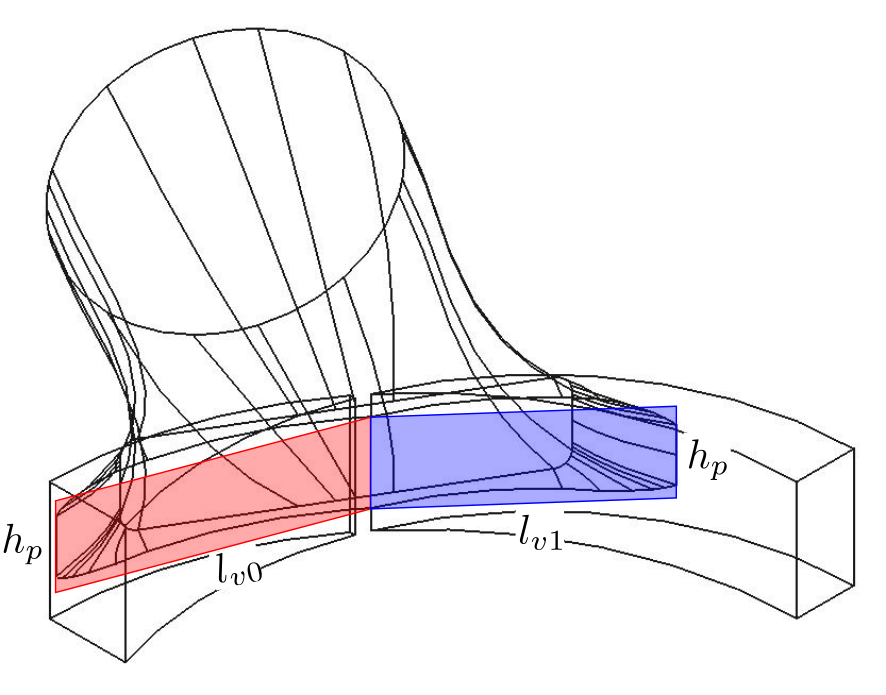
\includegraphics[]{area_referencia.png}
    \caption{Área de referencia}\label{fig:area_referencia}
\end{figure}

Tanto al inicio como al cierre del puerto ocurre solape de cámaras, por lo que
en estos intervalos angulares hay un valor de $C_D$ para cada cámara.
%
Este se calcula con el flujo másico que atraviesa los parches correspondientes
a cada cámara y el área de puerto expuesta por cada cámara.
% TODO: ver nota 8

\subsection{Interfaz con optimizador}
%
Para lograr ejecutar el simulador automáticamente, se hizo una librería de
funaciones capaz de tomar como dato de entrada un archivo de configuración que
incluye geometría, velocidades a ejecutar y cantidad de ciclos de simulación
entre otros.
%



\subsection{Ejecución del simulador}
%
Para permitir ejecutar el simulador directamente desde el algoritmo genético
se modificó ligeramente la forma de ejecutar el mismo.
%
El archivo de configuración de ICESym se pasa a través de un archivo
serializado de Python de tipo \emph{pickle}

\subsection{Salida de datos}
\subsection{Configuración adicional}
